% !TeX root = ../Notizen.tex

\section*{Aufgabe 2: Feigenbaum-Konstante)}
 In dieser Aufgabe wird die Feigenbaum-Konstante mithilfe der logistischen Abbildung bestimmen \cref{eq:logistik}.
 Dabei wird die Verkettung
 \begin{align*}
	f(f(f(\cdots f(r,x_0))))=f^{(2^n)}(r,x)
 \end{align*}
 definiert.
 Dazu wird der superstabile Fixpunkt $x^*=\frac{1}{2}=f^{(2^n)}(r,\frac{1}{2})$ betrachtet.
\subsection*{a)}
	Es wird zunächst die Funktion 
	\begin{align*}
		g_n(r)=\frac{1}{2}-f^{(2^n)}(r,\frac{1}{2})
	\end{align*}
	geplottet um Grenzen für die Nullstellen zu finden.
	\begin{figure}[h!]
		\centering
		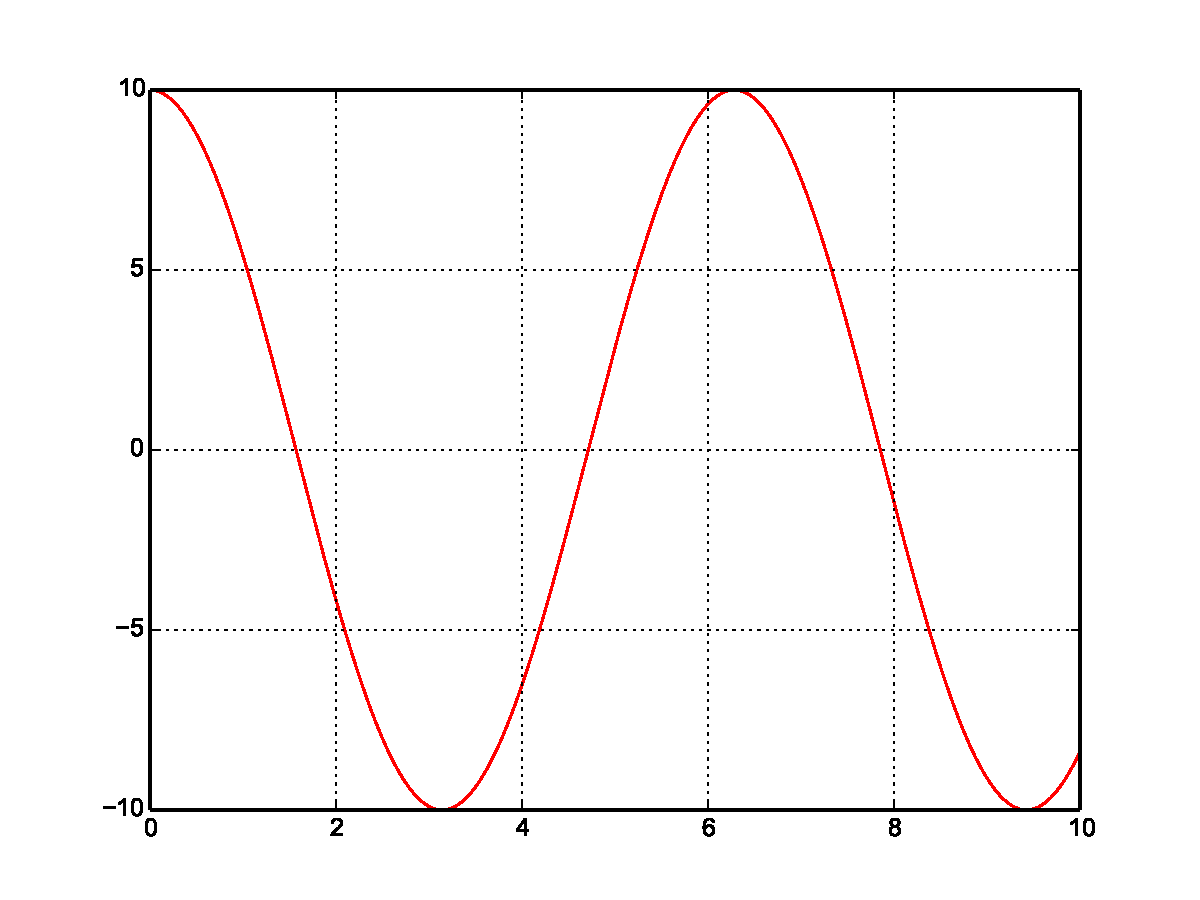
\includegraphics[width = \textwidth]{../Plots/Plot_2_A.pdf}
		\caption{Hier ist die Funktion für den superstabilen Fixpunkt dargestellt, sowie in die Grenzen für die Nullstellen.}
	\end{figure}
%plt.axvline( 1.9 , ls = "--" , color ="b" )
%plt.axvline( 2.1 , ls = "--" , color ="b" )
%plt.axvline( 3.2 , ls = "--" , color ="g" )
%plt.axvline( 3.25 , ls = "--" , color ="g")
%plt.axvline( 3.48 , ls = "--" , color ="r" )
%plt.axvline( 3.50 , ls = "--" , color ="r")
%plt.axvline( 3.54 , ls = "--" , color ="c" )
%plt.axvline( 3.56 , ls = "--" , color ="c")
Die Grenzen sind
\begin{align*}
	n=&0:\ r_\text{min}=1,90,\ r_\text{max}=2,10\\
	n=&1:\ r_\text{min}=3,20,\ r_\text{max}=3.25\\
	n=&2:\ r_\text{min}=3.48,\ r_\text{max}=3,50\\
	n=&3:\ r_\text{min}=3,54,\ r_\text{max}=3.56
\end{align*}
\subsection*{b)}
	Diese Grenzen können nun da zu verwendet werden um die Nullstellen der Funktion $g_n(r)$ zu bestimmen.
	Diese werden mithilfe des Refula Falsi bestimmt.
	Dazu müssen Zwei Start Werte $x_0<y_0$ der gewählt werden so das gilt $f(x_0)\cdot f(y_0)< 0$, also ein Vorzeichenwechsel statt findet. 
	Danach wird 
	\begin{align*}
		z_{n+1}=\frac{x_nf(y_n)-y_nf(x_n)}{f(y_n)-f(x_n)}
	\end{align*}
	Dann wird 
	\begin{align*}
	f(z_{n+1})f(x_n)\begin{cases}
		<0 \text{ dann wird } x_{n+1}=x_n\text{ und } y_{n+1}=z_{n+1}\\
		\text{ sonst }y_{n+1}=y_n\text{ und } x_{n+1}=z_{n+1}
	\end{cases}
	\end{align*}
	Danach wird die Änderung zwischen $x_n$ und $y_n$ bestimmt und wenn sie nicht kleiner ist als $10^{-7}$, dann wird das Verfahren wiederholt mit $x_n$ und $y_n$ als neue Startwerte.
	Daraus ergibt sich:
	\begin{align*}
	n=0:& R_0=2\\
	n=1:& R_1=3,23554\\
	n=2:& R_2=3,4984\\
	n=3:& R_3=3,55212
	\end{align*}
	\subsection*{c)}
	Zum Schluss wird eine erste Nährung für die Feigenbaum konstante 
	\begin{align*}
		\delta = \lim\limits_{n\to\infty}\frac{R_{n-1}-R_{n_2}}{R_{n}-R_{n-1}}
	\end{align*}
	bestimmt, durch $n\to3$.
	Die Feigenbaum-Konstante ergibt sich zu
	\begin{align*}
		\delta = 4,89344
	\end{align*} 
	